\chapter{شبیه‌سازی الگوریتم‌ها و پروتکل‌های کوانتومی}
در مورد این مساله که ذات مکانیک کوانتومی پیچیده است شکی نداریم. مساله‌ای که از آن پیچیده‌تر به نظر می‌رسد، الگوریتم‌های کوانتومی هستند. شهود بشریت با مسائلی مانند توپ و اهرم سازگارتر از مفاهیمی مانند الکترون و فوتون است و به نظر می‌رسد اتفاقاتی که در دنیای کوانتومی رخ می‌دهد چیزی شبیه جادو باشد. اما با کمی درنگ متوجه می‌شویم که همانند فیزیک کلاسیک، فیزیک کوانتومی از یک سری قائده و اصول مشخص پیروی می‌کند. اصولی که با بهره‌برداری هوشمندانه به بشریت در محاسبات، شبیه‌سازی و ... قدرتی بیش از پیش می‌دهد. برای ما، اولین قدم برای درک این قدرت محاسبات کوانتومی است. 
\section{مدار کوانتومی}
در دنیای کلاسیک، هر اطلاعاتی را می‌توان به صورت بیت‌های $0$ و $1$ نشان داد. همجنین، محاسبات را می‌توان از طریق مدارهای دیجیتالی پیش‌ برد. مداری مانند \autoref{fig:9-1} را به یاد بیاورید. 
\begin{figure}[h]
	\caption{مدار دیجیتالی ساده}
	\centering
	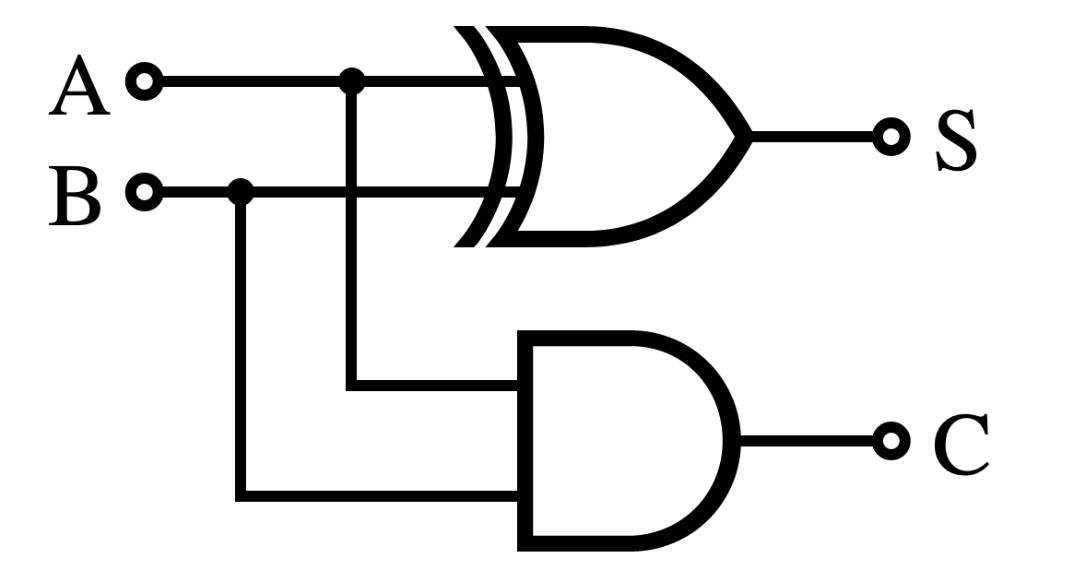
\includegraphics[width=10cm]{9_1.png}
	\label{fig:9-1}
\end{figure}
در مورد دنیای محاسبات کوانتومی نیز همین مساله صادق است. مثلا مدار کوانتومی \autoref{fig:9-2} کار مدار دیجیتالی شکل\ref{fig:9-1} را انجام می‌دهد. که همان جمع دو بیت و یا دو کیوبیت است. 
\begin{figure}[h]
	\caption{مدار کوانتومی ساده}
	\centering
	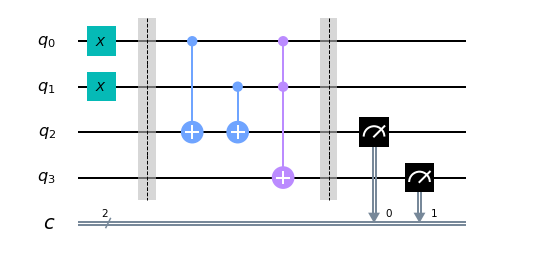
\includegraphics[width=10cm]{9_2.png}
	\label{fig:9-2}
\end{figure}
ابزاری که در ادامه برای شبیه‌سازی مفاهیم و الگوریتم‌های کوانتومی استفاده می‌کنیم کتابخانه پایتون $qisikit$
\cite{Qiskit}  محصول شرکت $IBM$ از پیشروهای علم محاسبات کوانتومی است. 
\subsection{اندازه‌گیری}
در شکل کد \ref{fig:9-3} تلاش می‌کنیم یک مدار کوانتومی ساده با اندازه اولیه $8$ کیوبیت که همه در حالت $\ket{0}$ بسازیم و سپس آن‌ها را اندازه بگیریم. 
\begin{figure}[h]
	\caption{ساخت مدار کوانتومی با $8$ کیوبیت و سپس اندازه‌گیری}
	\centering
	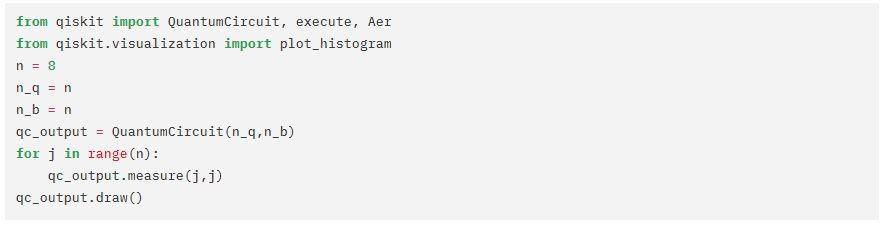
\includegraphics[width=15cm]{9_3.png}
	\label{fig:9-3}
\end{figure}
شکل مدار به صورت \ref{fig:9-4} خواهد بود. به نمادی که برای اندازه‌گیری مشخص می‌کنیم توجه کنید. 
 \begin{figure}[h]
	\caption{مدار کوانتومی اندازه‌گیری}
	\centering
	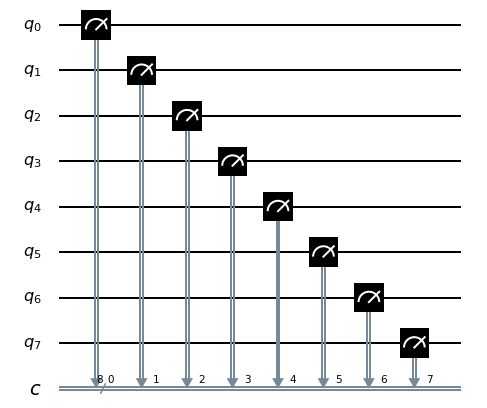
\includegraphics[width=10cm]{9_4.png}
	\label{fig:9-4}
\end{figure}
توجه کنید که کامپیوتر‌های کوانتومی و محاسبات کوانتومی شامل مقداری رفتار تصادفی هستند. به همین منظور، گاها نتایج چندین بار تکرار می‌شود تا به صورت آماری-احتمالی نتایج بررسی شود. مانند \autoref{fig:9-5}.
 \begin{figure}[h]
	\caption{بردار نتایج  بعد از چندبار اجرا}
	\centering
	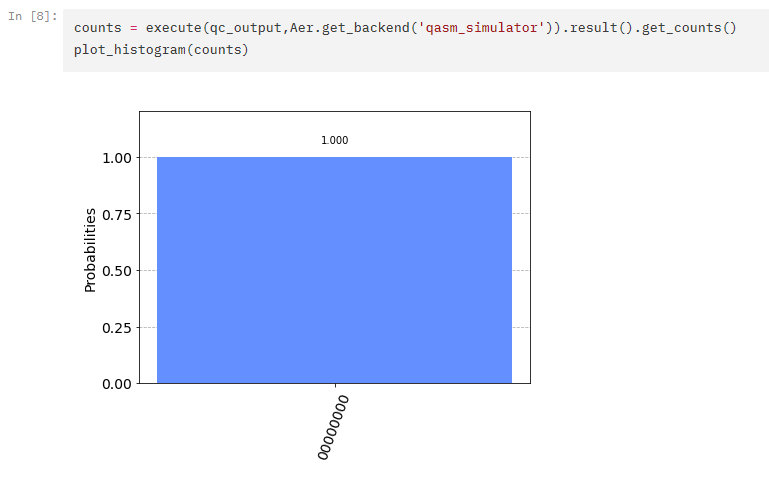
\includegraphics[width=10cm]{9_5.png}
	\label{fig:9-5}
\end{figure}
همچنین خوب است بدانیم که چون این ماشین‌های کلاسیک هستند که عملکرد ماشین کوانتومی را شبیه‌سازی می‌کنند، توانایی بیشتر از $30$ کیوبیت محاسبه را ندارند. 
\subsection{مدار جمع‌کننده}
برای طراحی مدارهای بیشتر، لازم است که با گیت‌های بیشتری آشنا شویم. به یاد داریم که گفته بودیم هر گیت کوانتومی یک عملگر یکانی است. پس عملگرهای یکانی مانند 
\begin{equation}
	  X = \begin{pmatrix} 0 & 1 \\ \\ 1 & 0 \end{pmatrix} 
\end{equation}
\begin{equation}
	  Z = \begin{pmatrix} 0 & 1 \\ \\ 1 & 0 \end{pmatrix} 
	\end{equation}
\begin{equation}
	  H =\frac{1}{\sqrt{2}} \begin{pmatrix} 1 & 1 \\ \\ 1 & -1 \end{pmatrix}  \\
\end{equation}
\begin{equation}
	 CX = \begin{pmatrix} 1 & 0 & 0 & 0 \\ \\ 0 & 1 & 0 & 0 \\ \\ 0 & 0 & 0 & 1 \\ \\ 0 & 0 & 1 & 0 \end{pmatrix}
\end{equation}
همه گیت‌های منطقی کوانتومی برگشت‌پذیر هستند. توجه کنید که عملگر دو کیوبیتی $CX$ یا نات-کنترل‌شده\footnote{Controlled-Not} عملگری است که برای هر دو کیوبیت ورودی، اگر کیوبیت اولیه برابر با $1$ باشد، خروجی دوم را $NOT$ ورودی دوم قرار می‌دهد و بالعکس. همچنین خروجی اول با ورودی اول برابر است. به  \autoref{fig:9-6} توجه کنید. ِ
\begin{figure}[h]
	\caption{گیت $CX$}
	\centering
	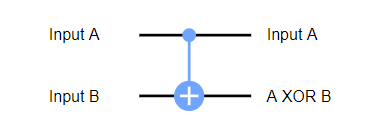
\includegraphics[width=10cm]{9_6.png}
	\label{fig:9-6}
\end{figure}
همانطور که می‌بینید، این عملگر همان $XOR$ است، اما برگشت‌پذیر هم هست‌! نکته‌ای که در دنیای دیجیتال نداریم. 

حال لازم است که یک گیت $AND$ هم داشته باشیم که برگشت‌پذیر هم باشد. گیت کوانتومی معادلی آن، گیت $Toffoli$ است  که روی فضای $3$ کیوبیت اعمال می‌شود. 
\begin{equation}
	CCX = \begin{pmatrix}
	1 & 0 & 0 & 0 & 0 & 0 & 0 & 0 \\ \\
	0 & 1 & 0 & 0 & 0 & 0 & 0 & 0 \\ \\
	0 & 0 & 1 & 0 & 0 & 0 & 0 & 0 \\ \\
	0 & 0 & 0 & 1 & 0 & 0 & 0 & 0 \\ \\
	0 & 0 & 0 & 0 & 1 & 0 & 0 & 0 \\ \\
	0 & 0 & 0 & 0 & 0 & 1 & 0 & 0 \\ \\
	0 & 0 & 0 & 0 & 0 & 0 & 0 & 1 \\ \\
	0 & 0 & 0 & 0 & 0 & 0 & 1 & 0
	\end{pmatrix}
\end{equation}
این گیت، اگر دو کیوبیت ورودی اول $1$ باشند، خروجی $1$ می‌دهند. 

حال لازم است مدار را بسازیم:
\begin{enumerate}
	\item لازم است که دو بیت اول با هم $XOR$ بشوند تا بیت کم ارزش مشخص شود.
	\item  برای مشخص کردن بیت پر ارزش هم لازم است که دو کیوبیت با هم $AND$ بشوند. 
	 \item برای این‌کار‌ها، 4 کیوبیت تعریف می‌کنیم. دو ورودی، دو خروجی و دو بیت کلاسیک برای اندازه گیری.   
\end{enumerate}
کد \autoref{fig:9-7} قرار است دو کیوبیت در حالت  $\ket{1}$ و $\ket{1}$ را جمع کند. 
\begin{figure}[h]
	\caption{کد مدار جمع‌کننده }
	\centering
	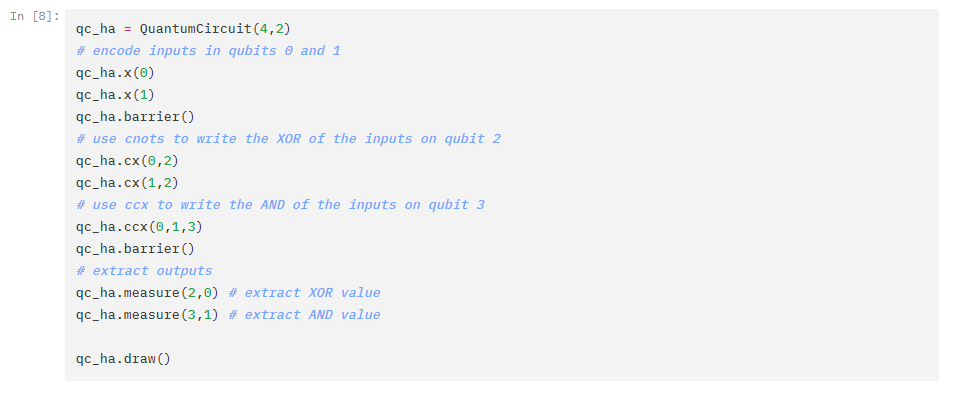
\includegraphics[width=15cm]{9_7.png}
	\label{fig:9-7}
\end{figure}
مدار نهایی در شکل \ref{fig:9-8} نشان داده شده است. مانند حالت پیشین تعدادی بار این کار را تکرار می‌کنیم تا نتیجه را ببینم. (شکل \ref{fig:9-9})
\begin{figure}[h]
	\caption{مدار جمع‌کننده}
	\centering
	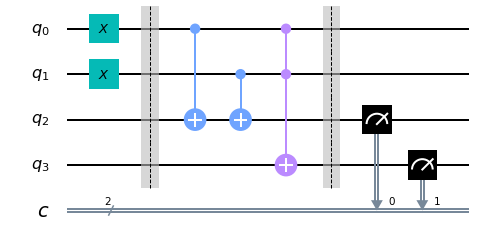
\includegraphics[width=10cm]{9_8.png}
	\label{fig:9-8}
\end{figure}
\begin{figure}[h]
	\caption{تکرار مدار}
	\centering
	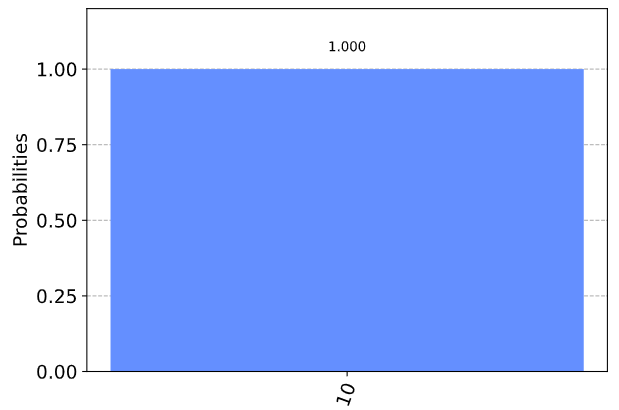
\includegraphics[width=6cm]{9_9.png}
	\label{fig:9-9}
\end{figure}
\section{فرابرد کوانتومی}
در این مرحله، یک کد ساده برای اجرای فرابرد کوانتومی اجرا می‌کنیم. مراحل کار را به یاد می‌آوریم:
\begin{enumerate}
	\item ابتدا آلیس و باب می‌بایست دو کیوبیت درهم‌تنیده در اشتراک بگذارند.
	\item آلیس عملگر هادامارد را روی کیوبیتی که می‌خواهد ارسال کند، اجرا می‌کند. 
	\item آلیس مقدار کیوبیت خود و کیوبیت ارسالی را اندازه می‌گیرد. 
	\item  مقدارهای به دست آمده را در اختیار باب می‌گذارد.
	\item باب با توجه به مقادیر به دست آمده، عملگرهای مختلف را روی کیوبیت خودش اعمال می‌کند.
\end{enumerate}
در شکل \ref{fig:9-10} کد مربوط به این کار را می‌بینید. در \autoref{fig:9-11} که مدار نهایی را نشان می‌دهد، کیوبیت اول بنا است که ارسال شود. کیوبیت دوم و سوم در‌هم‌تنیده شده‌اند و کیوبیت دوم در اختیار آلیس و کیوبیت سوم در اختیار باب است. در نهایت، نتیجه اندازه‌گیری آلیس بر روی دو ثبات کلاسیک می‌نشیند که در اختیار باب است و با توجه به نتیجه آن‌ها، عملگرهای $X$ و $Z$ را روی کیوبیت خود اجرا می‌کند. 
\begin{figure}[h]
	\caption{کد مدار فرابرد کوانتومی}
	\centering
	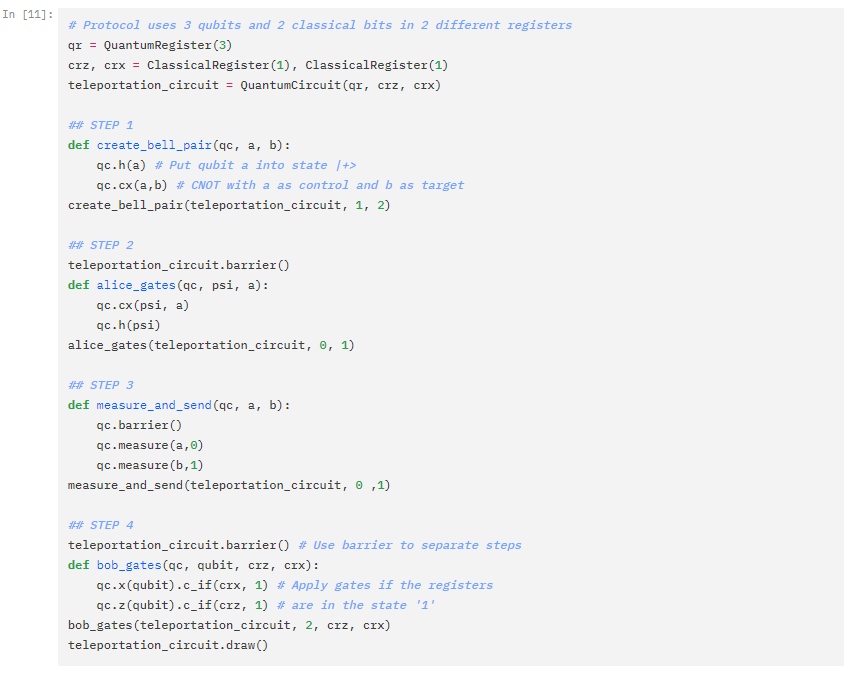
\includegraphics[width=15cm]{9_10.png}
	\label{fig:9-10}
\end{figure}
شکل مدار به صورت \ref{fig:9-11} است. 

\begin{figure}[h]
	\caption{ مدار فرابرد کوانتومی}
	\centering
	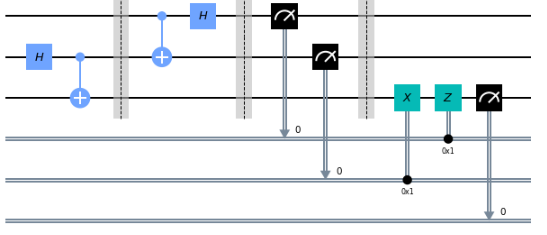
\includegraphics[width=10cm]{9_11.png}
	\label{fig:9-11}
\end{figure}
در نهایت با اندازه‌گیری حالت باب در یک ثبات دیگر می‌توانیم ببینم چگونه آخرین کیوبیت اندازه‌گیری شده همواره $0$ است. 
\begin{figure}[h]
	\caption{نتیجه اجرای کد به تعداد زیاد}
	\centering
	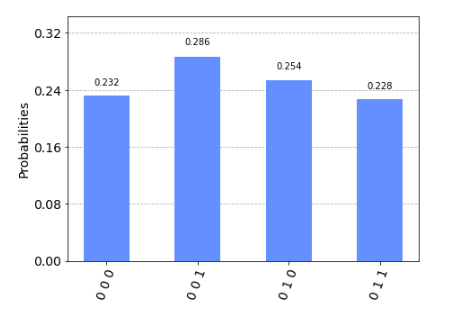
\includegraphics[width=10cm]{9_12.png}
	\label{fig:9-12}
\end{figure}

\section{الگوریتم دوچ-جوزا}
برای یادآوری، مراحل زیر یک اجرای الگوریتم دوچ-جوزا برای تشخیص ثابت یا مجموع صفر بودن تابع $f$ است. 
\begin{enumerate}
	\item دو ثبات کوانتومی آماده می‌کنیم. یکی با $n$ بیت و دیگری با $1$ بیت. اولی را با $0$ مقداردهی اولیه می‌کنیم و دومی را با $1$. 
	\begin{equation}
		\ket{\psi_{0}} = \ket{0}^{\otimes 0}\ket{1}
	\end{equation}
	\item سپس عملگرد هادامارد را روی هر کیوبیت اجرا می‌کنیم. 
	\begin{equation}
		\ket{\psi_{1}} = \frac{1}{\sqrt{2^{n+1}}} \sum_{x=0}^{2^{n}-1} \ket{x}(\ket{0}-\ket{1})
	\end{equation}
	\item جعبه‌ سیاه تابع $f$ را به این صورت اعمال می‌کنیم که در شکل\ref{fig:9-18} نشان داده شده است.
	\begin{equation}
		\begin{split}
		\ket{\psi_{2}} & = \frac{1}{\sqrt{2^{n+1}}} \sum_{x=0}^{2^{n}-1} \ket{x}(\ket{f(x)}-\ket{f(x) \oplus 1}) \\
		& = \frac{1}{\sqrt{2^{n+1}}} \sum_{x=0}^{2^{n}-1} (-1)^{f(x)}\ket{x}(\ket{0}-\ket{1})
		\end{split}
	\end{equation}
	\item در این مرحله، کیوبیت دوم را حذف می‌کنیم و یک بار دیگر هادامارد را اعمال می‌کنیم.  
\begin{equation}
		\begin{split}
		\ket{\psi_{3}} & = \frac{1}{2^{n}} \sum_{x=0}^{2^{n}-1} (-1)^{f(x)}   [\sum_{y=0}^{2^{n}-1} (-1)^{x.y}\ket{y} ]\\
		& = \frac{1}{2^{n}} \sum_{y=0}^{2^{n}-1} [\sum_{x=0}^{2^{n}-1} (-1)^{f(x)} (-1)^{x.y} ]\ket{y} \\
		\end{split}
	\end{equation}
	\item در نهایت با اندازه‌گیری کلیه کیوبیت‌ها، نتیجه‌گیری می‌کنیم. 
\end{enumerate}

\begin{figure}[h]
	\caption{چعبه‌سیاه تابع $f$ }
	\centering
	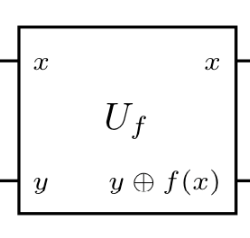
\includegraphics[width=5cm]{9_18.png}
	\label{fig:9-18}
\end{figure} 

در مرحله اول، تلاش می‌کنیم که یک جعبه‌سیاه برای این تابع بسازیم. بدین منظور، لازم است که شکل تابع را مشخص کنیم. فرض کنید عملیات را روی $4$ کیوبیت انجام می‌دهیم. در شکل  \ref{fig:9-13}، دقیقا عملیاتی که در مرحله سوم الگوریتم بالا رخ داد انجام شده است. در این تابع، یک تابع مجموع صفر را برنامه نویسی می‌کنیم.
\begin{figure}[h]
	\caption{کد دوچ-جوزا - جعبه سیاه}
	\centering
	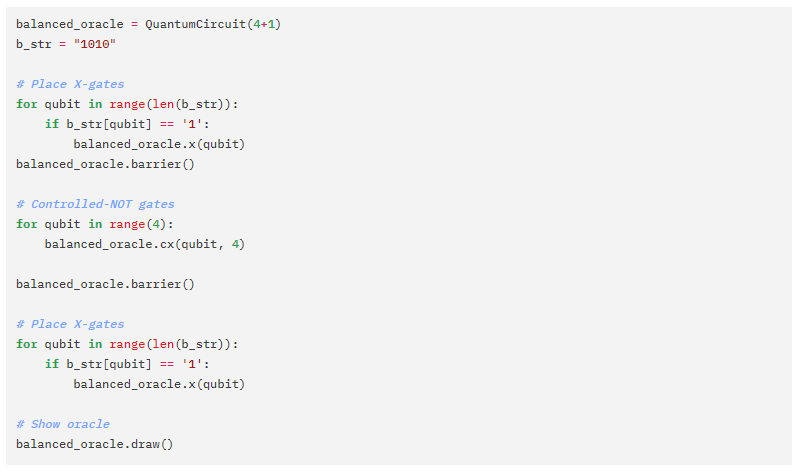
\includegraphics[width=15cm]{9_13.png}
	\label{fig:9-13}
\end{figure}  
که شکل \ref{fig:9-14} این مدار را نشان می‌دهد. 
\begin{figure}[h]
	\caption{مدار دوچ-جوزا - جعبه سیاه}
	\centering
	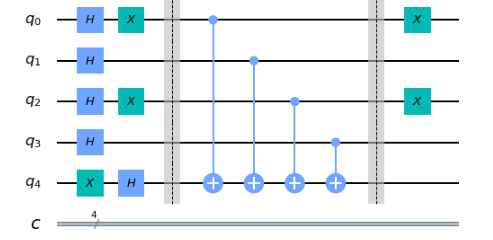
\includegraphics[width=10cm]{9_14.png}
	\label{fig:9-14}
\end{figure}
در ادامه، لازم است ورودی‌ها را بچینیم و مرحله $1$ و $2$ را انجام دهیم. سپس جعبه سیاه را وصله کنیم و مرحله $4$ و $5$ را اعمال کنیم. برای اینکار به شکل \ref{fig:9-15} توجه کنید. 
 
\begin{figure}[h]
	\caption{کد دوچ-جوزا }
	\centering
	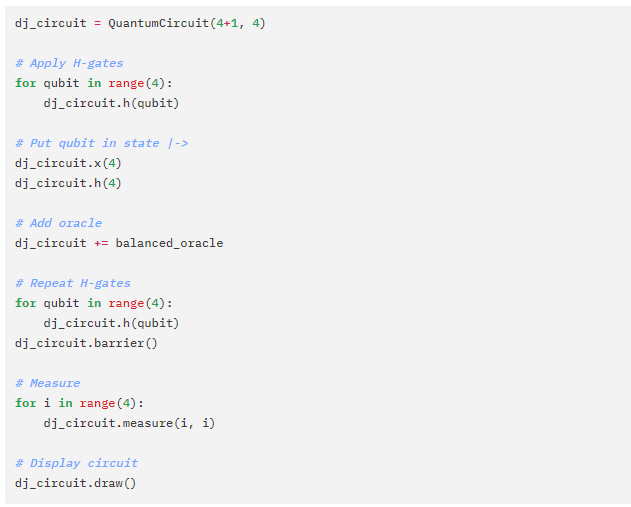
\includegraphics[width=12cm]{9_15.png}
	\label{fig:9-15}
\end{figure}
که مدار آن را در شکل \ref{fig:9-16} می‌بینیم. 
\begin{figure}[h]
	\caption{مدار دوچ-جوزا }
	\centering
	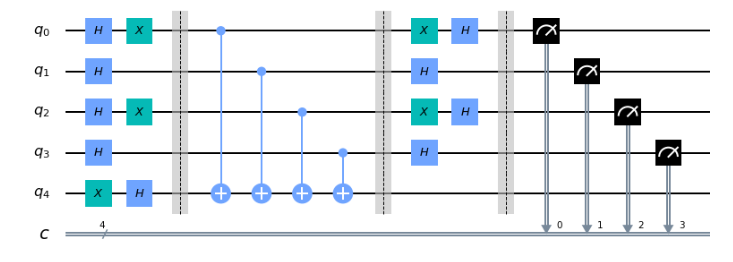
\includegraphics[width=12cm]{9_16.png}
	\label{fig:9-16}
\end{figure}
در نهایت، اجرای چندباره این الگوریتم با این تابع نشان ‌می‌دهد احتمال گرفتن $0000$ در خروجی $0$ است. (شکل \ref{fig:9-17})
\begin{figure}[h]
	\centering
	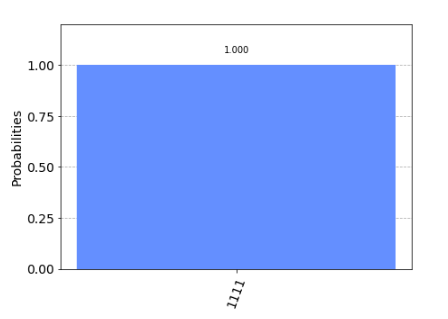
\includegraphics[width=6cm]{9_17.png}
	\caption{نتیجه اجرای چند باره الگوریتم دوچ جوزا. احتمال خروجی 1111 برابر با 100\% به‌دست آمده است.}
	\label{fig:9-17}
\end{figure}
\pagebreak
\section{الگوریتم دوچ-جوزا توزیع‌شده}

در ادامه قسمت قبل، الگوریتم ارائه شده در \autoref{djd} را پیاده‌سازی می‌کنیم.

کد مربوط به این قسمت نسبت به کدهای قبلی‌ طویل‌تر است و ارائه قسمت به قسمت آن در این مجال ممکن نیست. در پیوست دوم (\autoref{ap2})، کل کد تکه به تکه به همراه مدار مربوط به هر قسمت به تفضیل بررسی خواهد شد.\\
 مدار نهایی و نتیجه اجرای کد، در شکل‌های \ref{fig:sim1} و \ref{fig:sim2} آورده‌شده است.
  \begin{figure}
  \centering
 
 \includegraphics[width=.8\linewidth]{output_11_0.png}
 \caption{نتیجه اجرای چندباره الگوریتم دوچ جوزا توزیع شده و ارتباط بین آلیس و باب با ورودی‌های متفاوت.}
 \label{fig:sim2}
 \end{figure}
 \begin{figure}
 \centering
 
 \includegraphics[width=.9\linewidth]{output_8_0.png}
 \caption{مدار نهایی استفاده شده توسط آلیس (بالا) و باب (پایین) در الگوریتم‌ دوچ جوزا توزیع‌شده.}
 \label{fig:sim1}
 \end{figure}
 
